\documentclass[12pt]{article}
\usepackage[UTF8]{ctex}
\usepackage{xeCJK}
\usepackage[margin=1in]{geometry}
\usepackage{graphicx} % For including figures
\usepackage{amsmath}  % For math fonts, symbols and environments
\usepackage{pgfgantt} % For Gantt charts
\usepackage[hidelinks]{hyperref} % For hyperlinks
\usepackage{enumitem} % For customizing lists
\definecolor{blue}{HTML}{74BBC9}
\definecolor{yellow}{HTML}{F7E967}
\usepackage{listings}
\usepackage{xcolor}
\usepackage{tocloft} % 导入tocloft包
\usepackage{zi4}
\usepackage{fontspec}
\usepackage{setspace} % For setting line spacing

\usepackage{booktabs} % For professional looking tables
\usepackage{array}    % For extended column definitions
\usepackage{amsfonts} % For math fonts like '\mathbb{}'
\usepackage{amssymb}  % For math symbols
\usepackage{caption}  % For custom captions
\usepackage[table]{xcolor} % For coloring tables
\usepackage{tabularx} % For auto-sized table columns
\usepackage{algorithm}

\usepackage{algpseudocode}
\usepackage{enumitem}
\usepackage{tikz}
\usetikzlibrary{positioning}

% 目录标题样式定义
\renewcommand{\cfttoctitlefont}{\hfill\Large\bfseries}
\renewcommand{\cftaftertoctitle}{\hfill\mbox{}\par}

% 设置中文主字体为宋体,指定相对路径
\setCJKmainfont[
    Path = ./,
    BoldFont = SimSun.ttc,
    ItalicFont = SimSun.ttc
]{SimSun.ttc}

% 设置英文主字体为Times New Roman
\setmainfont{Times New Roman}

% 设置正文格式:宋体,小四,行距20磅
\renewcommand\normalsize{%
    \CJKfamily{song}\fontsize{12pt}{20pt}\selectfont}

% Monokai theme with a lighter background
\definecolor{codegreen}{rgb}{0,0.6,0}
\definecolor{codegray}{rgb}{0.5,0.5,0.5}
\definecolor{codepurple}{rgb}{0.58,0,0.82}
\definecolor{backcolour}{rgb}{0.95,0.95,0.92}
\setmonofont{Source Code Pro}[Contextuals={Alternate}]

\lstdefinestyle{mystyle}{
    backgroundcolor=\color{backcolour},   
    commentstyle=\color{codegreen},
    keywordstyle=\color{magenta},
    numberstyle=\tiny\color{codegray},
    stringstyle=\color{codepurple},
    basicstyle=\ttfamily\footnotesize,
    breakatwhitespace=false,         
    breaklines=true,                 
    captionpos=b,                    
    keepspaces=true,                 
    numbers=left,                    
    numbersep=5pt,                  
    showspaces=false,                
    showstringspaces=false,
    showtabs=false,                  
    tabsize=2
}

\lstset{style=mystyle}

\title{\textbf{PR Experiment Report Collection}}
\author{58122204 谢兴}
\date{\today}

\begin{document}

\begin{titlepage}
  \begin{figure}[htbp]
    \centering
    
\includegraphics[scale=0.2]{figures/southeast_university_logo.png}
    % \caption{实际投掷距离与理想条件下投掷距离对比}
    \label{fig1}
  \end{figure}

  \centering
  \vspace*{40pt}
  \Huge\textbf{模式识别实验报告}

  \vspace{60pt}
  \Large
  % 专业:人工智能

  % \vspace{30pt}
  % 学号:58122204

  % \vspace{30pt}
  % 年级:大二

  % \vspace{30pt}
  % 姓名:谢兴


  % \vspace{30pt}
  % 签名:


  % \vspace{30pt}
  % 时间:\today
  \begin{center}

    % \begin{tabularx}{0.8\textwidth}{>{\raggedleft\arraybackslash}X >{\centering\arraybackslash}X}
    %   专业: & \underline{\makebox[6cm][c]{人工智能}} \\
    %   学号: & \underline{\makebox[6cm][c]{58122204}} \\
    %   年级: & \underline{\makebox[6cm][c]{大二}} \\
    %   姓名: & \underline{\makebox[6cm][c]{谢兴}} \\
    % \end{tabularx}
    \begin{table}[h]
      \centering
      \begin{Large}
        \begin{spacing}{1.5} % 设置行间距为1.5倍
          \begin{tabular}{p{1.5cm} p{6cm}<{\centering}}
            专业: & \underline{\makebox[6cm][c]{人工智能}}     \\
            学号: & \underline{\makebox[6cm][c]{58122204}} \\
            年级: & \underline{\makebox[6cm][c]{大二}}       \\
            姓名: & \underline{\makebox[6cm][c]{谢兴}}       \\
          \end{tabular}
        \end{spacing}
      \end{Large}
    \end{table}




    \vspace{5cm}

    \begin{flushright}
      \begin{tabularx}{0.4\textwidth}{>{\raggedleft\arraybackslash}X >{\centering\arraybackslash}X}
        签名: & \\
        时间: & \\
      \end{tabularx}
    \end{flushright}
  \end{center}
  %   \begin{center}
  %     \begin{tabular}{rl}
  %         专业: & \underline{\hspace{6cm}} \\
  %         学号: & \underline{\hspace{6cm}} \\
  %         年级: & \underline{\hspace{6cm}} \\
  %         姓名: & \underline{\hspace{6cm}} \\
  %     \end{tabular}
  % \end{center}

\end{titlepage}

\newpage
\tableofcontents

% 实验一
\newpage
\section{\centering 实验一 KNN Classification}

\subsection{问题描述}
\subsection{概述}
利用KNN算法,对 Iris 鸢尾花数据集中的测试集进行分类。
\subsection{任务说明}
\begin{enumerate}
  \item 利用欧式距离作为KNN算法的度量函数,对测试集
        进行分类。实验报告中,要求在验证集上分析近邻
        数$k$对KNN算法分类精度的影响。
  \item 利用马氏距离作为KNN算法的度量函数,对测试集
        进行分类。
  \item 基于MindSpore平台提供的官方模型库,对相同的
        数据集进行训练,并与自己独立实现的算法对比结
        果(包括但不限于准确率、算法迭代收敛次数等指
        标),并分析结果中出现差异的可能原因,给出使
        用MindSpore的心得和建议。
  \item (加分项)使用MindSpore平台提供的相似任务数
        据集(例如,其他的分类任务数据集)测试自己独
        立实现的算法并与MindSpore平台上的官方实现算
        法进行对比,并进一步分析差异及其成因。
\end{enumerate}

\subsection{实现步骤与流程}

\subsubsection{实验思路}
\begin{enumerate}
  \item 导入必要的库,包括 \texttt{numpy}, \texttt{pandas}, \texttt{matplotlib}, \texttt{plotly} 和 \texttt{seaborn};
  \item 数据加载和基本信息显示;
        \begin{enumerate}
          \item 从 \texttt{data/train.csv} 文件中加载训练数据集
          \item 显示数据集的前几行数据
          \item 显示数据集的描述性统计信息
          \item 显示数据集的基本信息,包括数据类型和缺失值情况
        \end{enumerate}
  \item 数据可视化;
        \begin{enumerate}
          \item 使用 \texttt{Seaborn} 绘制数据集的特征两两关系图,并按标签着色
          \item 使用 \texttt{Plotly} 绘制数据分布的饼图
          \item 分别绘制每个特征(萼片长度、萼片宽度、花瓣长度、花瓣宽度)的箱线图和直方图
        \end{enumerate}
  \item 实现基于Euiclidean距离和基于Mahalanobis距离的KNN算法;

  \item 数据处理和预测;
        \begin{enumerate}
          \item 加载测试数据集并进行必要的类型转换和缺失值检查
          \item 使用预训练模型对测试数据进行预测,并将预测结果保存到 \texttt{CSV} 文件中
        \end{enumerate}
  \item 最后对比欧式距离和马氏距离两种度量方式的分类效果和差异
        \begin{enumerate}
          \item 比较多个预测结果文件 \texttt{task1\_test\_prediction.csv} 和\\ \texttt{task2\_test\_prediction.csv}之间的差异,
                找出不同的行和列,并打印出不同值的位置
        \end{enumerate}
\end{enumerate}

\subsubsection{数学模型}
KNN算法的数学模型如下:

给定一个测试样本$x$,KNN算法通过计算$x$与训练集中所有样本之间的距离(常用欧氏距离),选择距离最近的$k$个样本,然后通过多数投票法决定$x$的类别。
欧氏距离的计算公式为:
\[
  d(x_1, x_2) = \sqrt{\sum_{i=1}^{n} (x_{1i} - x_{2i})^2}
\]

马氏距离的计算公式为:
\[d(x_1, x_2) = \sqrt{(x_1 - x_2)^T \Sigma^{-1} (x_1 - x_2)}\]
其中,$\Sigma$为协方差矩阵。


\subsubsection{关键难点}
\begin{enumerate}
  \item 如何高效地计算欧氏距离。
  \item 如何在较大的数据集上进行快速的邻居搜索。
  \item 如何处理训练数据和测试数据的维度一致性问题。
  \item 如何在分类时处理类别不均衡的问题。
\end{enumerate}


\subsubsection{算法描述}
基于Euiclidean距离和Mahalanobis距离的KNN算法的伪代码分别
见算法~\ref{K-Nearest Neighbors Based on Euclidean Distance} 和算法~\ref{K-Nearest Neighbors Based on Mahalanobis Distance}。

\begin{algorithm}
  \caption{K-Nearest Neighbors Based on Euclidean Distance}
  \label{K-Nearest Neighbors Based on Euclidean Distance}
  \begin{algorithmic}[1]
    \State 初始化KNN分类器,邻居数为$k$
    \Procedure{拟合}{X\_train, y\_train}
    \State 存储训练数据和标签
    \EndProcedure
    \Procedure{预测}{$X$}
    \For{每个测试数据$x$}
    \State 计算$x$与所有训练样本之间的欧氏距离
    \State 对距离进行排序,选择最近的$k$个邻居
    \State 对这$k$个邻居的标签进行多数投票
    \State 将多数投票结果赋予$x$
    \EndFor
    \State \Return 预测的标签
    \EndProcedure
  \end{algorithmic}
\end{algorithm}


\begin{algorithm}
  \caption{K-Nearest Neighbors Based on Mahalanobis Distance}
  \label{K-Nearest Neighbors Based on Mahalanobis Distance}
  \begin{algorithmic}[1]
    \State 初始化KNN分类器,邻居数为$k$,矩阵$A$的维度为$e$,学习率为$\eta$,最大迭代次数为$max\_iter$
    \Procedure{拟合}{X\_train, y\_train}
    \State 存储训练数据和标签
    \State 初始化矩阵$A$为随机值
    \For{迭代次数 $iteration = 1, 2, \ldots, max\_iter$}
    \State 初始化梯度矩阵$\nabla A$为零
    \For{每个训练样本 $x_i$}
    \State 获取与$x_i$同类的样本索引$same\_class\_indices$
    \For{每个同类样本 $x_j$}
    \If{$i == j$}
    \State 跳过
    \EndIf
    \State 计算$p_{ij}$值
    \State 计算样本差异$diff = x_i - x_j$
    \State 更新梯度$\nabla A += 2 \cdot p_{ij} \cdot (A \cdot diff) \cdot diff^T$
    \EndFor
    \EndFor
    \State 按学习率更新矩阵$A$: $A = A - \eta \cdot \nabla A / n$
    \EndFor
    \EndProcedure
    \Procedure{预测}{$X$}
    \For{每个测试数据$x$}
    \State 计算$x$与所有训练样本之间的马氏距离
    \State 对距离进行排序,选择最近的$k$个邻居
    \State 对这$k$个邻居的标签进行多数投票
    \State 将多数投票结果赋予$x$
    \EndFor
    \State \Return 预测的标签
    \EndProcedure
  \end{algorithmic}
\end{algorithm}

\subsubsection{马氏距离梯度计算公式推导}

假设我们有训练数据集$\{(x_i, y_i)\}_{i=1}^n$,其中$x_i \in \mathbb{R}^d$为样本特征,$y_i$为样本类别。为了优化马氏距离下的KNN算法,我们需要学习一个矩阵$A \in \mathbb{R}^{e \times d}$,使得同类样本之间的距离最小化。马氏距离的计算公式为:
\begin{equation}
  d_M(x_i, x_j) = \sqrt{(x_i - x_j)^\top A^\top A (x_i - x_j)}
\end{equation}

为了优化矩阵$A$,我们使用如下的目标函数:
\begin{equation}
  \mathcal{L} = \sum_{i=1}^n \sum_{j \in \mathcal{N}(i)} p_{ij} \cdot d_M^2(x_i, x_j)
\end{equation}
其中,$\mathcal{N}(i)$表示与$x_i$同类的样本索引集合,$p_{ij}$为权重,定义为:
\begin{equation}
  p_{ij} = \frac{\exp(-d_M^2(x_i, x_j))}{\sum_{k \in \mathcal{N}(i)} \exp(-d_M^2(x_i, x_k))}
\end{equation}

首先,我们对$d_M^2(x_i, x_j)$进行展开:
\begin{equation}
  d_M^2(x_i, x_j) = (x_i - x_j)^\top A^\top A (x_i - x_j)
\end{equation}

为了计算梯度$\nabla_A \mathcal{L}$,我们需要对$\mathcal{L}$关于$A$求导:
\begin{equation}
  \mathcal{L} = \sum_{i=1}^n \sum_{j \in \mathcal{N}(i)} p_{ij} (x_i - x_j)^\top A^\top A (x_i - x_j)
\end{equation}

对$A$求导时,需要使用链式法则:
\begin{equation}
  \frac{\partial \mathcal{L}}{\partial A} = \sum_{i=1}^n \sum_{j \in \mathcal{N}(i)} \left( \frac{\partial p_{ij}}{\partial A} (x_i - x_j)^\top A^\top A (x_i - x_j) + p_{ij} \frac{\partial ((x_i - x_j)^\top A^\top A (x_i - x_j))}{\partial A} \right)
\end{equation}

首先计算$p_{ij}$对$A$的导数。由于$p_{ij}$包含在指数函数内,我们得到:
\begin{equation}
  \frac{\partial p_{ij}}{\partial A} = p_{ij} \left( -\sum_{k \in \mathcal{N}(i)} p_{ik} \cdot 2(x_i - x_k)^\top A^\top \cdot (x_i - x_k) + 2(x_i - x_j)^\top A^\top \cdot (x_i - x_j) \right)
\end{equation}

然后计算$(x_i - x_j)^\top A^\top A (x_i - x_j)$对$A$的导数:
\begin{equation}
  \frac{\partial ((x_i - x_j)^\top A^\top A (x_i - x_j))}{\partial A} = 2 A (x_i - x_j) (x_i - x_j)^\top
\end{equation}

将以上结果代入梯度公式中,我们得到:
\begin{equation}
  \begin{aligned}
    \nabla_A \mathcal{L} = & \sum_{i=1}^n \sum_{j \in \mathcal{N}(i)} \left[ p_{ij} \left( -\sum_{k \in \mathcal{N}(i)} p_{ik} \cdot 2(x_i - x_k)^\top A^\top \cdot (x_i - x_k) \right. \right. \\
                           & \left. \left. + 2(x_i - x_j)^\top A^\top \cdot (x_i - x_j) \right) + 2 p_{ij} A (x_i - x_j) (x_i - x_j)^\top \right]
  \end{aligned}
\end{equation}

整理后得到最终的梯度公式:
\begin{equation}
  \nabla_A \mathcal{L} = 2 \sum_{i=1}^n \sum_{j \in \mathcal{N}(i)} p_{ij} \left[ A (x_i - x_j) (x_i - x_j)^\top - \sum_{k \in \mathcal{N}(i)} p_{ik} A (x_i - x_k) (x_i - x_k)^\top \right]
\end{equation}


\subsection{实验结果与分析}
\subsubsection{数据集的部分可视化分析}
\begin{enumerate}
  \item \texttt{train.csv}文件中训练数据的pairplot图如图~\ref{fig:pairplot} 所示。
  \item 训练数据的分布情况如图~\ref{fig:pie} 所示,可以看出这三类鸢尾花的数据分布比例是不完全一致的,但三类的数据量大致相同。
  \item
\end{enumerate}

\begin{figure}[htbp]
  \centering
  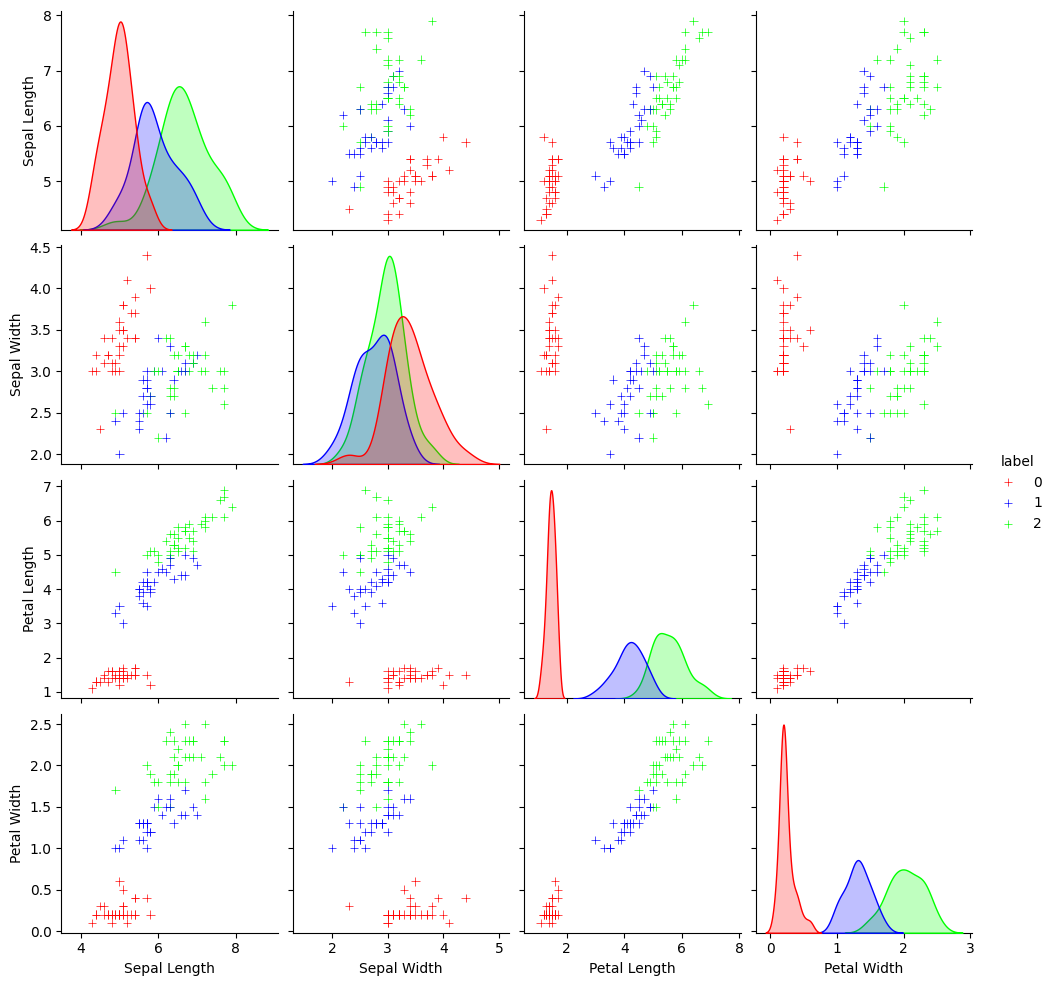
\includegraphics[scale=0.45]{figures/knn/pairplot.png}
  \caption{train.csv训练数据的pairplot图}
  \label{fig:pairplot}
\end{figure}

\begin{figure}[htbp]
  \centering
  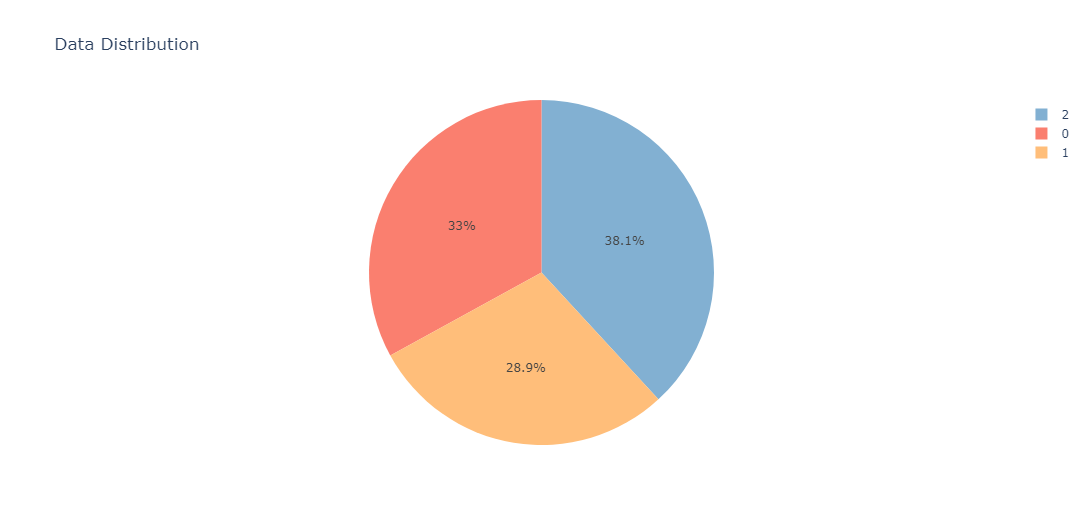
\includegraphics[scale=0.4]{figures/knn/distribution.png}
  \caption{train.csv训练数据分布比例}
  \label{fig:pie}
\end{figure}

\subsubsection{实验结果的分析}

\begin{enumerate}
  \item 对于基于欧氏距离的KNN算法,当$k=3$时,测试集的准确率为93.33\%;
  \item 对于基于马氏距离的KNN算法,当$k=3$时,测试集的准确率为93.33\%;
  \item 将$k$从1到50遍历,分析出基于欧氏距离的KNN算法对Iris数据集进行分类的准确率随$k$的变化情况,如图~\ref{fig:accuracy}所示。
\end{enumerate}
显然,基于欧式距离的最佳$k$值为5或27或29,此时的准确率最高,为100\%,说明$k=5$,$k=27$,$k=29$时能完全正确的将Iris数据集中三类鸢尾花进行分类。

\begin{figure}[htbp]
  \centering
  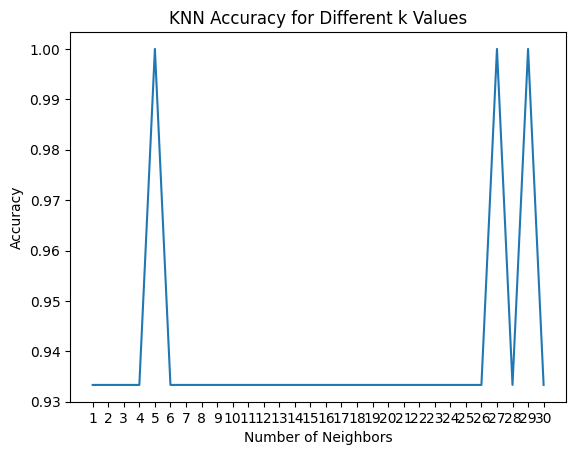
\includegraphics[scale=0.8]{figures/knn/accuracy.png}
  \caption{分类准确率随$k$的变化情况}
  \label{fig:accuracy}
\end{figure}



\subsection{MindSpore 学习使用心得体会}

\subsection{代码附录(数据加载可视化展示部分,具体见knn.ipynb文件)}
\subsubsection{\texttt{knn.ipynb}}
\begin{lstlisting}[language=Python]
# 实验一代码
\end{lstlisting}

\subsubsection{\texttt{knn\_mindspore.ipynb}}
\begin{lstlisting}[language=Python]
# 实验一代码
\end{lstlisting}

% 实验二
\newpage
\section{\centering 实验二 Na\"ive Bayes Classification}

\subsection{问题描述}
\subsubsection{概述}
利用朴素贝叶斯算法,对MNIST数据集中的测试集
进行分类。
\subsubsection{任务说明}

\begin{enumerate}
  \item 在课程学习中同学们已经学习了贝叶斯分类理论并掌握了其基本原理,即利用贝叶斯公式
        \[
          p(\omega_j|x) = \frac{p(x|\omega_j)p(\omega_j)}{p(x)}
        \]
        对\(p(\omega_j|x)\)作出预测。由于\(p(x)\)为一固定值,所以一般不在计算过程中求得\(p(x)\)的具体值。在实际运用中,为了方便计算,通常假设数据特征之间相互独立,即
        \[
          p(x|\omega_j) = p(x_1|\omega_j) \cdot p(x_2|\omega_j) \cdots p(x_d|\omega_j), \quad x \in \mathbb{R}^d,
        \]
        这便是著名的朴素贝叶斯算法。

  \item MNIST数据集本身以二进制形式保存,所以首先需要选择合适的编程语言编写读写二进制数据的程序完成对图片、标记信息的初步提取工作。读取了图片信息后,发现每个像素点的值在[0,1]区间内,这是图像压缩后的结果,所以可以先将像素值乘以255再取整,得到每一个点的灰度值。将图像二值化,得到可以用于分类的28×28个特征向量以及对应的标签数据,之后便可以交由贝叶斯分类器进行学习。

  \item 基于MindSpore平台提供的官方模型库,对相同的数据集进行训练,并与自己独立实现的算法对比结果(包括但不限于准确率、算法迭代收敛次数等指标),并分析结果中出现差异的可能原因,给出使用MindSpore的心得和建议。

  \item (加分项)使用MindSpore平台提供的相似任务数据集(例如,其他的分类任务数据集)测试自己独立实现的算法并与MindSpore平台上的官方实现算法进行对比,并进一步分析差异及其成因。
\end{enumerate}

\subsection{实现步骤与流程}
\subsubsection{实验思路}


\subsubsection{数学模型}


\subsubsection{关键难点}


\subsubsection{算法描述}
朴素贝叶斯算法实现的伪代码如算法~\ref{Optimized Multinomial Naive Bayes} 所示。
\begin{algorithm}
  \caption{Optimized Multinomial Naive Bayes}
  \label{Optimized Multinomial Naive Bayes}
  \begin{algorithmic}[1]
    \State \textbf{Input:} 平滑参数 $\alpha$
    \State \textbf{Initialize:}
    \State \quad 类别数 $n\_classes$
    \State \quad 特征数 $n\_features$
    \State \quad 类别计数 $class\_count$
    \State \quad 特征计数 $feature\_count$
    \State \quad 类别对数先验 $class\_log\_prior$
    \State \quad 特征对数概率 $feature\_log\_prob$

    \Procedure{拟合}{X, y}
    \State 获取唯一类别 $classes = \text{np.unique}(y)$
    \State 初始化类别计数 $class\_count$ 和特征计数 $feature\_count$
    \For{每个类别 $c \in classes$}
    \State 获取属于类别 $c$ 的样本 $X_c$
    \State 更新类别计数 $class\_count[c]$
    \State 更新特征计数 $feature\_count[c, :]$
    \EndFor
    \State 计算类别对数先验 $class\_log\_prior$
    \State 计算特征对数概率 $feature\_log\_prob$
    \EndProcedure

    \Procedure{预测}{X}
    \State 计算对数似然 $log\_likelihood = X \times feature\_log\_prob^T$
    \State 计算对数后验概率 $log\_posterior = log\_likelihood + class\_log\_prior$
    \State 返回类别 $classes[\text{np.argmax}(log\_posterior, axis=1)]$
    \EndProcedure

  \end{algorithmic}
\end{algorithm}
\subsubsection{}

\subsection{实验结果与分析}

\subsection{MindSpore 学习使用心得体会}

\subsection{代码附录}

\begin{lstlisting}[language=Python]
# 实验二代码
\end{lstlisting}

% 实验三
\newpage
\section{\centering 实验三 Neural Network Image Classification}

\subsection{问题描述}
\subsection{概述}
利用神经网络算法,对CIFAR数据集中的测试集进
行分类。
\subsection{任务说明}
\begin{enumerate}%[label=\(\Box\)]
  \item 基于神经网络模型及BP算法,根据训练集中的数据对你设计的神经网络模型进行训练,随后对给定的打乱的测试集中的数据进行分类。

  \item 基于MindSpore平台提供的官方模型库,对相同的数据集进行训练,并与自己独立实现的算法对比结果(包括但不限于准确率、算法迭代收敛次数等指标),并分析结果中出现差异的可能原因。

  \item (加分项)使用MindSpore平台提供的相似任务数据集(例如,其他的分类任务数据集)测试自己独立实现的算法并与MindSpore平台上的官方实现算法进行对比,并进一步分析差异及其成因。
\end{enumerate}

\subsection{实现步骤与流程}
\subsubsection{实验环境}
实验环境见表~\ref{tab:indicators}。

\begin{table}[!t]
  \caption{Experiment Environment}
  \label{tab:indicators}
  \centering
  \begin{tabular}{m{5cm}<{\centering}m{5cm}<{\centering}m{4cm}<{\centering}}
    \toprule
    \textbf{Items}   & \textbf{Version}     \\[\medskipamount]
    \midrule
    CPU              & Intel Core i5-1135G7 \\[\medskipamount]
    RAM              & 16 GB                \\[\medskipamount]
    Python           & 3.11.5               \\[\medskipamount]
    % scikit-learn     & 1.3.2                \\[\medskipamount]
    Operating system & Windows11            \\[\medskipamount]
    \bottomrule
  \end{tabular}
\end{table}

\subsubsection{实验思路}
\begin{enumerate}
  \item \textbf{数据加载与预处理}:
        \begin{enumerate}
          \item 从CIFAR-10数据集中加载图像数据和标签。
          \item 将图像数据从原始格式转换为适用于神经网络的格式(32 $\times$ 32 $\times$ 3 $\rightarrow$ 3072)。
          \item 将图像数据进行归一化处理,将像素值缩放到[0, 1]范围内。
        \end{enumerate}

  \item \textbf{数据划分}:
        \begin{enumerate}
          \item 将加载的训练数据划分为训练集和验证集,以便在训练过程中进行模型评估。
        \end{enumerate}

  \item \textbf{定义全连接神经网络结构}:
        \begin{enumerate}
          \item 输入层:包含3072个神经元,对应每张图像的3072个像素值。
          \item 隐藏层:包含100个神经元,使用ReLU激活函数。
          \item 输出层:包含10个神经元,对应10个类别,使用Softmax激活函数。
        \end{enumerate}

  \item \textbf{定义前向传播与反向传播}:
        \begin{enumerate}
          \item 前向传播:计算输入数据通过网络后的输出。
          \item 反向传播:根据预测结果和实际标签计算损失,并更新网络权重。
        \end{enumerate}

  \item \textbf{模型训练}:
        \begin{enumerate}
          \item 使用小批量梯度下降(Mini-Batch Gradient Descent)优化网络权重。
          \item 在每个epoch结束后,计算并记录训练损失、验证损失和验证准确率。
        \end{enumerate}

  \item \textbf{模型评估}:
        \begin{enumerate}
          \item 在测试集上评估模型性能,计算并输出测试集准确率。
          \item 绘制训练过程中损失和准确率的变化曲线。
        \end{enumerate}

  \item \textbf{混淆矩阵}:
        \begin{enumerate}
          \item 计算混淆矩阵,分析分类结果的具体表现。
          \item 绘制混淆矩阵,直观展示模型在各个类别上的分类效果。
        \end{enumerate}
  \item \textbf{预测结果展示}
        \begin{enumerate}
          \item 展示模型在测试集部分图片上的分类结果。
        \end{enumerate}
\end{enumerate}
本实验的超参数如表~\ref{tab:training-params} 所示。
\begin{table}[htbp]
  \centering
  \caption{训练参数}
  \label{tab:training-params}
  \begin{tabular}{m{3cm}<{\centering}m{3cm}<{\centering}}
    \toprule
    \textbf{参数}   & \textbf{值}    \\[\medskipamount]
    \midrule
    learning rate & 0.01          \\[\medskipamount]
    epochs        & 100           \\[\medskipamount]
    % optimizer     & SGD           \\[\medskipamount]
    loss function & Cross Entropy \\[\medskipamount]
    performance   & accuracy      \\[\medskipamount]
    batch size    & 64            \\[\medskipamount]
    num\_hiddens  & 128           \\[\medskipamount]
    \bottomrule
  \end{tabular}
\end{table}


\subsubsection{数学模型}
BP神经网络的数学模型如图~\ref{fig:fcnn_structure} 所示。
\tikzset{%
  neuron missing/.style={
      draw=none,
      scale=4,
      text height=0.333cm,
      execute at begin node=\color{black}$\vdots$
    },
}
\begin{figure}[htbp]
  \centering
  \begin{tikzpicture}[x=1.5cm, y=1.5cm, >=stealth]

    \foreach \m/\l [count=\y] in {1,2,3}
      {
        \node [circle,fill=green!50,minimum size=1cm] (input-\m) at (0,2.5-\y) {};
      }
    \foreach \m/\l [count=\y] in {4}
      {
        \node [circle,fill=green!50,minimum size=1cm ] (input-\m) at (0,-2.5) {};
      }

    \node [neuron missing]  at (0,-1.5) {};


    \foreach \m [count=\y] in {1}
    \node [circle,fill=red!50,minimum size=1cm ] (hidden-\m) at (2,0.75) {};

    \foreach \m [count=\y] in {2}
    \node [circle,fill=red!50,minimum size=1cm ] (hidden-\m) at (2,-1.85) {};

    \node [neuron missing]  at (2,-0.3) {};


    \foreach \m [count=\y] in {1}
    \node [circle,fill=blue!50,minimum size=1cm ] (output-\m) at (4,1.5-\y) {};

    \foreach \m [count=\y] in {2}
    \node [circle,fill=blue!50,minimum size=1cm ] (output-\m) at (4,-0.5-\y) {};

    \node [neuron missing]  at (4,-0.4) {};

    \foreach \l [count=\i] in {1,2,3, 3072}
    \draw [<-] (input-\i) -- ++(-1,0)
    node [above, midway] {$I_{\l}$};

    \foreach \l [count=\i] in {1,128}
    \node [above] at (hidden-\i.north) {$H_{\l}$};

    \foreach \l [count=\i] in {1,10}
    \draw [->] (output-\i) -- ++(1,0)
    node [above, midway] {$O_{ \l}$};

    \foreach \i in {1,...,4}
    \foreach \j in {1,...,2}
    \draw [->] (input-\i) -- (hidden-\j);

    \foreach \i in {1,...,2}
    \foreach \j in {1,...,2}
    \draw [->] (hidden-\i) -- (output-\j);

    %\foreach \l [count=\x from 0] in {Input, Hidden, Output}
    % \node [align=center, above] at (\x*2,2) {\l \\ layer};

  \end{tikzpicture}
  \caption{全连接神经网络结构示意图}
  \label{fig:fcnn_structure}
\end{figure}


\subsubsection{关键难点}
在训练过程中实时评估模型的性能,并根据评估结果调整模型的超参数,如学习率、批次大小、隐藏层神经元数量等。
需要平衡模型的复杂度和泛化能力,避免过拟合或欠拟合。

\subsubsection{算法描述}
使用BP神经网络训练算法,如算法~\ref{FullyConnectedNN Training Algorithm} 所示。
% \begin{algorithm}
%   \caption{BP神经网络训练算法}
%   \label{BP Neural Network Training Algorithm}
%   \begin{algorithmic}[1]
%     \State 初始化网络的权重$\mathbf{W}$和偏置$\mathbf{b}$为随机值
%     \Procedure{训练}{X, y, x\_val, y\_val, batch\_size, learning\_rate, epochs}
%       \For{每个epoch}
%         \For{每个mini-batch}
%           \State \textbf{前向传播}:
%           \State \quad 设输入$\mathbf{x}$
%           \State \quad 计算每一层的输出和激活值:
%           \State \quad \quad $\mathbf{z}^{(l)} = \mathbf{W}^{(l)} \mathbf{a}^{(l-1)} + \mathbf{b}^{(l)}$
%           \State \quad \quad $\mathbf{a}^{(l)} = \sigma(\mathbf{z}^{(l)})$
%           \State \quad 其中,$\sigma$为激活函数
%           \State \textbf{计算损失}:
%           \State \quad 使用损失函数计算输出层的损失$L$
%           \State \textbf{反向传播}:
%           \State \quad 计算输出层的误差:
%           \State \quad \quad $\delta^{(L)} = \mathbf{a}^{(L)} - \mathbf{y}$
%           \State \quad 计算隐藏层的误差:
%           \State \quad \quad $\delta^{(l)} = (\mathbf{W}^{(l+1)})^T \delta^{(l+1)} \odot \sigma'(\mathbf{z}^{(l)})$
%           \State \quad 计算梯度:
%           \State \quad \quad $\nabla_{\mathbf{W}^{(l)}} = \delta^{(l)} (\mathbf{a}^{(l-1)})^T$
%           \State \quad \quad $\nabla_{\mathbf{b}^{(l)}} = \delta^{(l)}$
%           \State \textbf{更新权重和偏置}:
%           \State \quad $\mathbf{W}^{(l)} = \mathbf{W}^{(l)} - \eta \nabla_{\mathbf{W}^{(l)}}$
%           \State \quad $\mathbf{b}^{(l)} = \mathbf{b}^{(l)} - \eta \nabla_{\mathbf{b}^{(l)}}$
%         \EndFor
%         \State 计算训练集和验证集的准确率
%       \EndFor
%     \EndProcedure
%   \end{algorithmic}
% \end{algorithm}

\begin{algorithm}
  \caption{全连接神经网络训练算法}
  \label{FullyConnectedNN Training Algorithm}
  \begin{algorithmic}[1]
    \State 初始化网络的权重$\mathbf{W1}, \mathbf{W2}$和偏置$\mathbf{b1}, \mathbf{b2}$为随机值
    \Procedure{训练}{X\_train, Y\_train, X\_val, Y\_val, batch\_size, learning\_rate, epochs}
    \For{每个epoch}
    \For{每个mini-batch}
    \State \textbf{前向传播}:
    \State \quad 设输入$\mathbf{X}$
    \State \quad 计算第一层的输出和激活值:
    \State \quad \quad $\mathbf{Z1} = \mathbf{X} \mathbf{W1} + \mathbf{b1}$
    \State \quad \quad $\mathbf{A1} = \max(0, \mathbf{Z1})$ \Comment{ReLU激活函数}
    \State \quad 计算第二层的输出和激活值:
    \State \quad \quad $\mathbf{Z2} = \mathbf{A1} \mathbf{W2} + \mathbf{b2}$
    \State \quad \quad $\mathbf{A2} = \text{softmax}(\mathbf{Z2})$
    \State \textbf{计算损失}:
    \State \quad 使用交叉熵损失函数计算损失$L$
    \State \textbf{反向传播}:
    \State \quad 计算输出层的误差$\delta^{(2)}$
    \State \quad 计算隐藏层的误差$\delta^{(1)}$
    \State \quad 计算梯度:
    \State \quad \quad $\nabla_{\mathbf{W2}} = \mathbf{A1}^T \delta^{(2)}$
    \State \quad \quad $\nabla_{\mathbf{b2}} = \sum \delta^{(2)}$
    \State \quad \quad $\nabla_{\mathbf{W1}} = \mathbf{X}^T \delta^{(1)}$
    \State \quad \quad $\nabla_{\mathbf{b1}} = \sum \delta^{(1)}$
    \State \textbf{更新权重和偏置}:
    \State \quad 使用学习率$\eta$更新$\mathbf{W1}, \mathbf{b1}, \mathbf{W2}, \mathbf{b2}$
    \EndFor
    \State 计算训练集和验证集的损失和准确率
    \EndFor
    \EndProcedure
  \end{algorithmic}
\end{algorithm}

\subsection{实验结果与分析}

\begin{enumerate}
  \item \textbf{准确率曲线}
        本实验训练集和验证集上的准确率随epoch的变化曲线如图~\ref{fig:accuracy_curve} 所示。
        从图中可以看出,随着epoch的增加,验证集的准确率逐渐提高,最终收敛到\textbf{50\%}。
  \item \textbf{损失曲线}
        本实验验证集上的损失随epoch的变化曲线如图~\ref{fig:loss_curve} 所示。
        从图中可以看出,随着epoch的增加,训练接和验证集的损失逐渐降低,最终收敛到一个稳定值。
        其中训练集损失稳定在\textbf{1.0}左右,验证集损失稳定在\textbf{1.4}左右。
  \item \textbf{混淆矩阵}
        本实验的混淆矩阵如图~\ref{fig:confusion_matrix}所示。
        从图中可以看出,模型在不同类别上的分类效果,以及各类别之间的混淆情况。
\end{enumerate}


\begin{figure}[htbp]
  \centering
  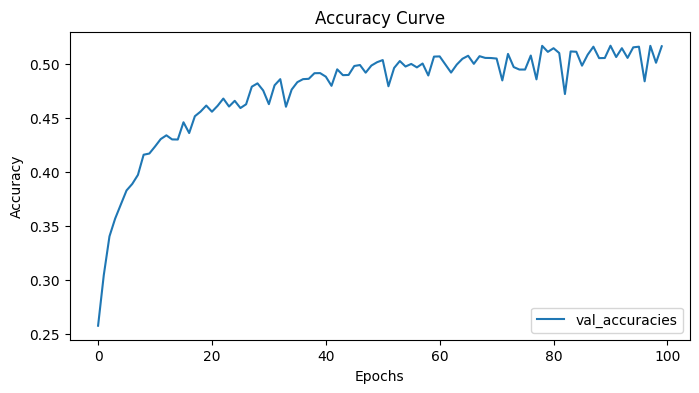
\includegraphics[scale=0.75]{figures/nn/accuracy_curve.png}
  \caption{Accuracy随epoch的变化曲线}
  \label{fig:accuracy_curve}
\end{figure}

\begin{figure}[htbp]
  \centering
  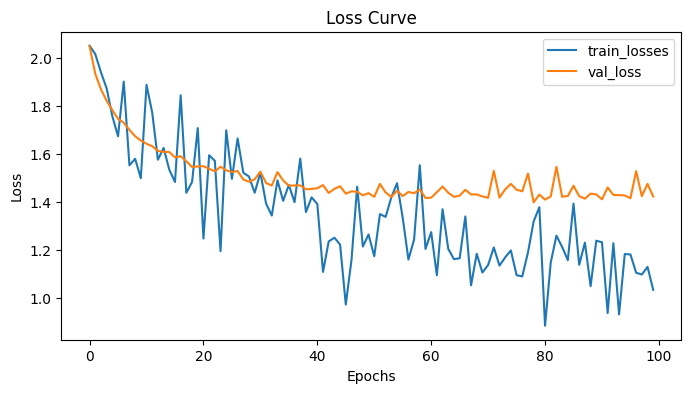
\includegraphics[scale=0.75]{figures/nn/loss_curve.png}
  \caption{Loss随epoch的变化曲线}
  \label{fig:loss_curve}
\end{figure}


\begin{figure}[htbp]
  \centering
  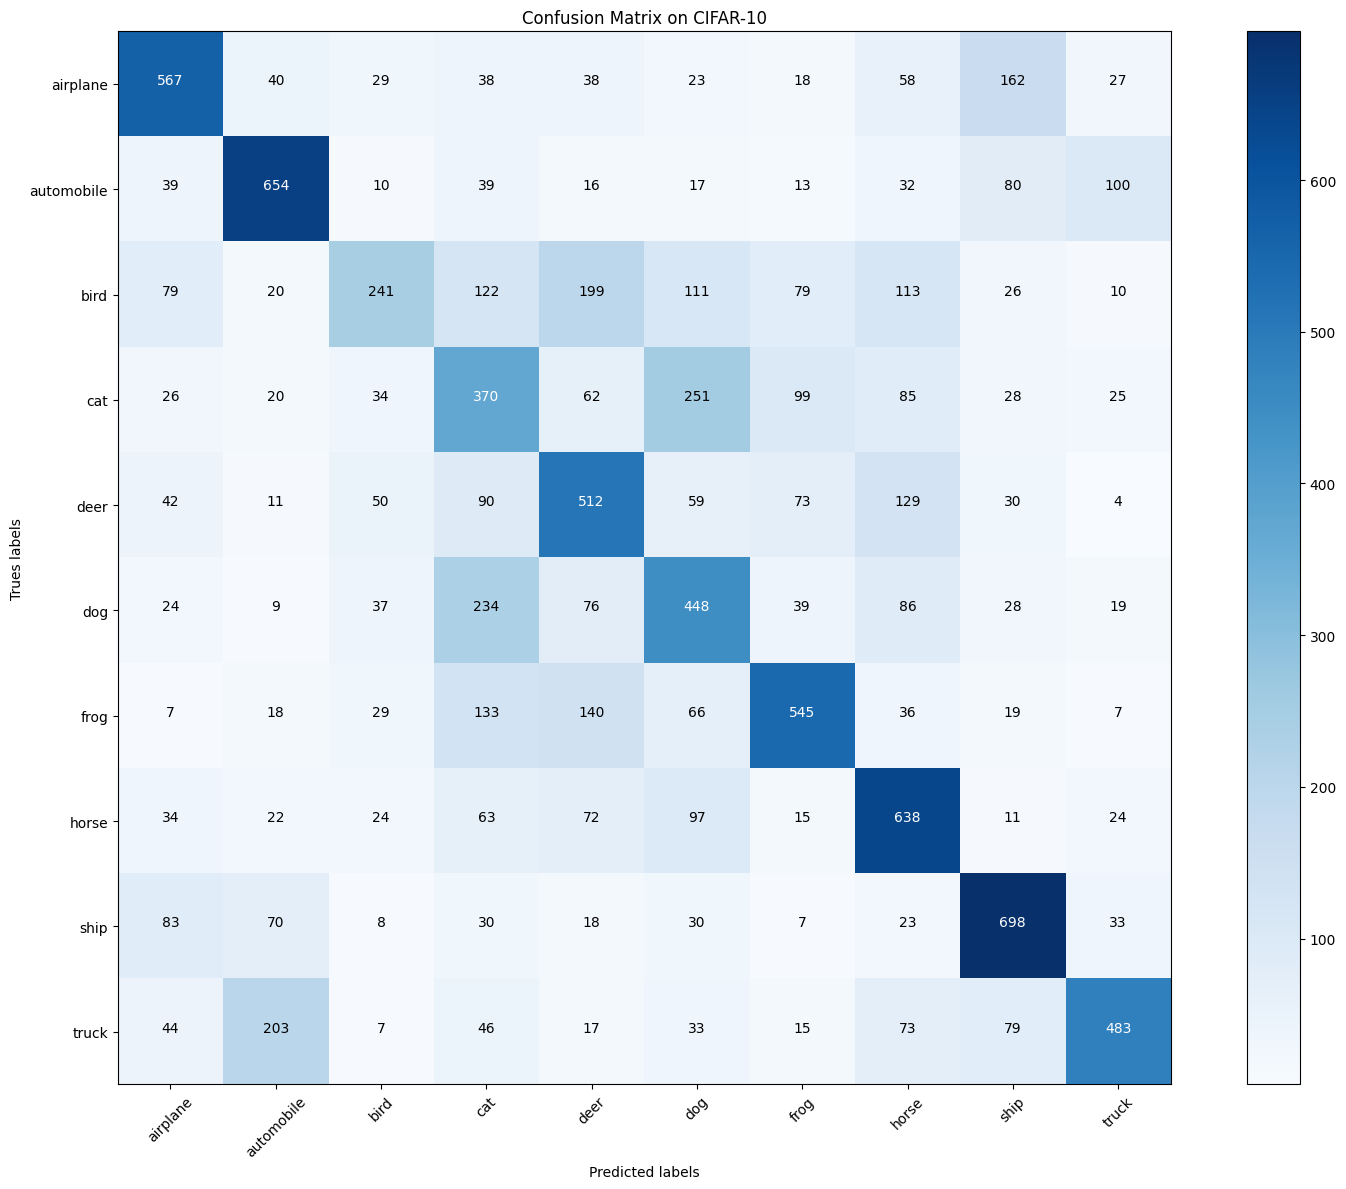
\includegraphics[scale=0.5]{figures/nn/confusion_matrix.png}
  \caption{Confusion Matrix on CIFAR-10}
  \label{fig:confusion_matrix}
\end{figure}


\subsection{MindSpore 学习使用心得体会}

\subsection{代码附录}

\subsubsection{\texttt{cifar-10-scratch.ipynb}}
\begin{lstlisting}[language=Python]
  import pickle
  import numpy as np
  import os
  import matplotlib.pyplot as plt
  
  # 加载 CIFAR-10 批次数据
  def load_cifar10_batch(filename):
      with open(filename, 'rb') as f:
          datadict = pickle.load(f, encoding='bytes')
          X = datadict[b'data']
          Y = datadict[b'labels']
          X = X.reshape(10000, 3, 32, 32).astype("float")
          Y = np.array(Y)
          return X, Y
  
  # 加载所有 CIFAR-10 数据
  def load_cifar10(ROOT):
      xs = []
      ys = []
      for b in range(1, 6):
          f = os.path.join(ROOT, 'data_batch_%d' % (b,))
          X, Y = load_cifar10_batch(f)
          xs.append(X)
          ys.append(Y)
      Xtr = np.concatenate(xs)
      Ytr = np.concatenate(ys)
      del X, Y
      Xte, Yte = load_cifar10_batch(os.path.join(ROOT, 'test_batch'))
      return Xtr, Ytr, Xte, Yte
  
  ROOT = './cifar-10-batches-py'
  X_train, y_train, X_test, y_test = load_cifar10(ROOT)
  
  # 全连接神经网络类
  class FullyConnectedNN:
      def __init__(self, input_size, hidden_size, output_size):
          self.W1 = np.random.randn(input_size, hidden_size) * 0.01
          self.b1 = np.zeros((1, hidden_size))
          self.W2 = np.random.randn(hidden_size, output_size) * 0.01
          self.b2 = np.zeros((1, output_size))
  
      def relu(self, Z):
          return np.maximum(0, Z)
  
      def softmax(self, Z):
          expZ = np.exp(Z - np.max(Z))
          return expZ / expZ.sum(axis=1, keepdims=True)
  
      def forward(self, X):
          self.Z1 = np.dot(X, self.W1) + self.b1
          self.A1 = self.relu(self.Z1)
          self.Z2 = np.dot(self.A1, self.W2) + self.b2
          self.A2 = self.softmax(self.Z2)
          return self.A2
  
      def compute_loss(self, Y, Y_hat):
          m = Y.shape[0]
          log_likelihood = -np.log(Y_hat[range(m), Y])
          loss = np.sum(log_likelihood) / m
          return loss
  
      def backward(self, X, Y, Y_hat):
          m = X.shape[0]
          dZ2 = Y_hat
          dZ2[range(m), Y] -= 1
          dZ2 /= m
  
          dW2 = np.dot(self.A1.T, dZ2)
          db2 = np.sum(dZ2, axis=0, keepdims=True)
  
          dA1 = np.dot(dZ2, self.W2.T)
          dZ1 = dA1 * (self.Z1 > 0)
  
          dW1 = np.dot(X.T, dZ1)
          db1 = np.sum(dZ1, axis=0, keepdims=True)
  
          self.W1 -= self.learning_rate * dW1
          self.b1 -= self.learning_rate * db1
          self.W2 -= self.learning_rate * dW2
          self.b2 -= self.learning_rate * db2
  
      def compute_accuracy(self, X, Y):
          Y_hat = self.forward(X)
          predictions = np.argmax(Y_hat, axis=1)
          accuracy = np.mean(predictions == Y)
          return accuracy
  
      def train(self, X_train, Y_train, X_val, Y_val, epochs=300, learning_rate=0.01):
          self.learning_rate = learning_rate
          train_losses = []
          val_losses = []
          val_accuracies = []
  
          for epoch in range(epochs):
              # 打乱训练数据
              indices = np.arange(X_train.shape[0])
              np.random.shuffle(indices)
              X_train = X_train[indices]
              Y_train = Y_train[indices]
  
              # 小批量梯度下降
              for start_idx in range(0, X_train.shape[0], batch_size):
                  end_idx = min(start_idx + batch_size, X_train.shape[0])
                  X_batch = X_train[start_idx:end_idx]
                  Y_batch = Y_train[start_idx:end_idx]
  
                  # 前向传播
                  Y_hat_train = self.forward(X_batch)
                  train_loss = self.compute_loss(Y_batch, Y_hat_train)
                  
                  # 反向传播
                  self.backward(X_batch, Y_batch, Y_hat_train)
  
              # 每个 epoch 结束后计算验证集上的损失和准确率
              Y_hat_val = self.forward(X_val)
              val_loss = self.compute_loss(Y_val, Y_hat_val)
              val_accuracy = self.compute_accuracy(X_val, Y_val)
              
              # 存储损失和准确率
              train_losses.append(train_loss)
              val_losses.append(val_loss)
              val_accuracies.append(val_accuracy)
              
              # 打印每个 epoch 的损失和准确率
              print(f'Epoch [{epoch + 1}], train_loss: {train_loss:.4f}, val_loss: {val_loss:.4f}, val_acc: {val_accuracy:.4f}')
          
          return train_losses, val_losses, val_accuracies
  
  # 预处理数据
  X_train = X_train.reshape(X_train.shape[0], -1) / 255.0
  X_test = X_test.reshape(X_test.shape[0], -1) / 255.0
  
  # 将训练数据分成训练集和验证集
  split_index = int(0.8 * X_train.shape[0])
  X_val, y_val = X_train[split_index:], y_train[split_index:]
  X_train, y_train = X_train[:split_index], y_train[:split_index]
  
  # 超参数
  input_size = 3072  # 32*32*3
  hidden_size = 100
  output_size = 10
  learning_rate = 0.01
  epochs = 100
  batch_size = 64
  
  # 初始化并训练模型
  model = FullyConnectedNN(input_size, hidden_size, output_size)
  train_losses, val_losses, val_accuracies = model.train(X_train, y_train, X_val, y_val, epochs, learning_rate)
  
  # 在测试集上进行预测
  y_pred = np.argmax(model.forward(X_test), axis=1)
  accuracy = np.mean(y_pred == y_test)
  print(f'测试集准确率: {accuracy:.4f}')
  
  # 绘制损失曲线
  epochs_range = range(epochs)
  plt.figure(figsize=(8, 4))
  plt.plot(epochs_range, train_losses, label='训练损失')
  plt.plot(epochs_range, val_losses, label='验证损失')
  plt.xlabel('Epochs')
  plt.ylabel('Loss')
  plt.legend(loc='upper right')
  plt.title('损失曲线')
  plt.show()
  
  # 绘制准确率曲线
  plt.figure(figsize=(8, 4))
  plt.plot(epochs_range, val_accuracies, label='验证准确率')
  plt.xlabel('Epochs')
  plt.ylabel('Accuracy')
  plt.legend(loc='lower right')
  plt.title('准确率曲线')
  plt.show()
  
  
  # 计算混淆矩阵
  def compute_confusion_matrix(y_true, y_pred, num_classes):
      cm = np.zeros((num_classes, num_classes), dtype=int)
      for i in range(len(y_true)):
          cm[y_true[i], y_pred[i]] += 1
      return cm
  
  # 绘制混淆矩阵
  def plot_confusion_matrix(cm, classes, title='混淆矩阵', cmap=plt.cm.Blues):
      plt.figure(figsize=(16, 12))
      plt.imshow(cm, interpolation='nearest', cmap=cmap)
      plt.title(title)
      plt.colorbar()
      tick_marks = np.arange(len(classes))
      plt.xticks(tick_marks, classes, rotation=45)
      plt.yticks(tick_marks, classes)
  
      fmt = 'd'
      thresh = cm.max() / 2.
      for i, j in np.ndindex(cm.shape):
          plt.text(j, i, format(cm[i, j], fmt),
                   horizontalalignment="center",
                   color="white" if cm[i, j] > thresh else "black")
  
      plt.ylabel('真实标签')
      plt.xlabel('预测标签')
      plt.tight_layout()
      plt.show()
  
  # CIFAR-10 标签
  cifar10_labels = ['airplane', 'automobile', 'bird', 'cat', 'deer', 'dog', 'frog', 'horse', 'ship', 'truck']
  
  # 计算并绘制混淆矩阵
  cm = compute_confusion_matrix(y_test, y_pred, len(cifar10_labels))
  plot_confusion_matrix(cm, classes=cifar10_labels)
  
\end{lstlisting}

\newpage
\section{\centering 心得体会}

\subsection{关于上课的体会}

\subsection{关于实验的体会}

\subsection{总的体会}

\end{document}
